\subsection{Factory Method}

\subsubsection*{Problembeschreibung}

Es wird ein Interface benötigt, um eine Reihe von konkreten Produkten erzeugen zu können. Jedes konkrete Produkt hat jedoch andere Anforderungen an seine eigene Erzeugung. Eine Factory-Method kann eingesetzt werden, wenn eine Klasse kein Wissen darüber besitzt oder besitzen soll, welches konkrete Produkt sie zu erzeugen hat oder eine Klasse die Verantwortlichkeit über diese Entscheidung ihren Subklassen überlassen möchte.

\subsubsection*{Lösung}

Es existiert ein eine abstrakte `Creator`-Klasse, welche ein Interface bereitstellt, um Produkte zu erzeugen. Die Details der Erzeugung dieser Produkte sind in den konkreten Subklassen von `Creator` implementiert. Jeder konkrete `Creator` kann somit einen Typ von konkretem Produkt erschaffen.

\begin{figure}[!hb]
	\centering
	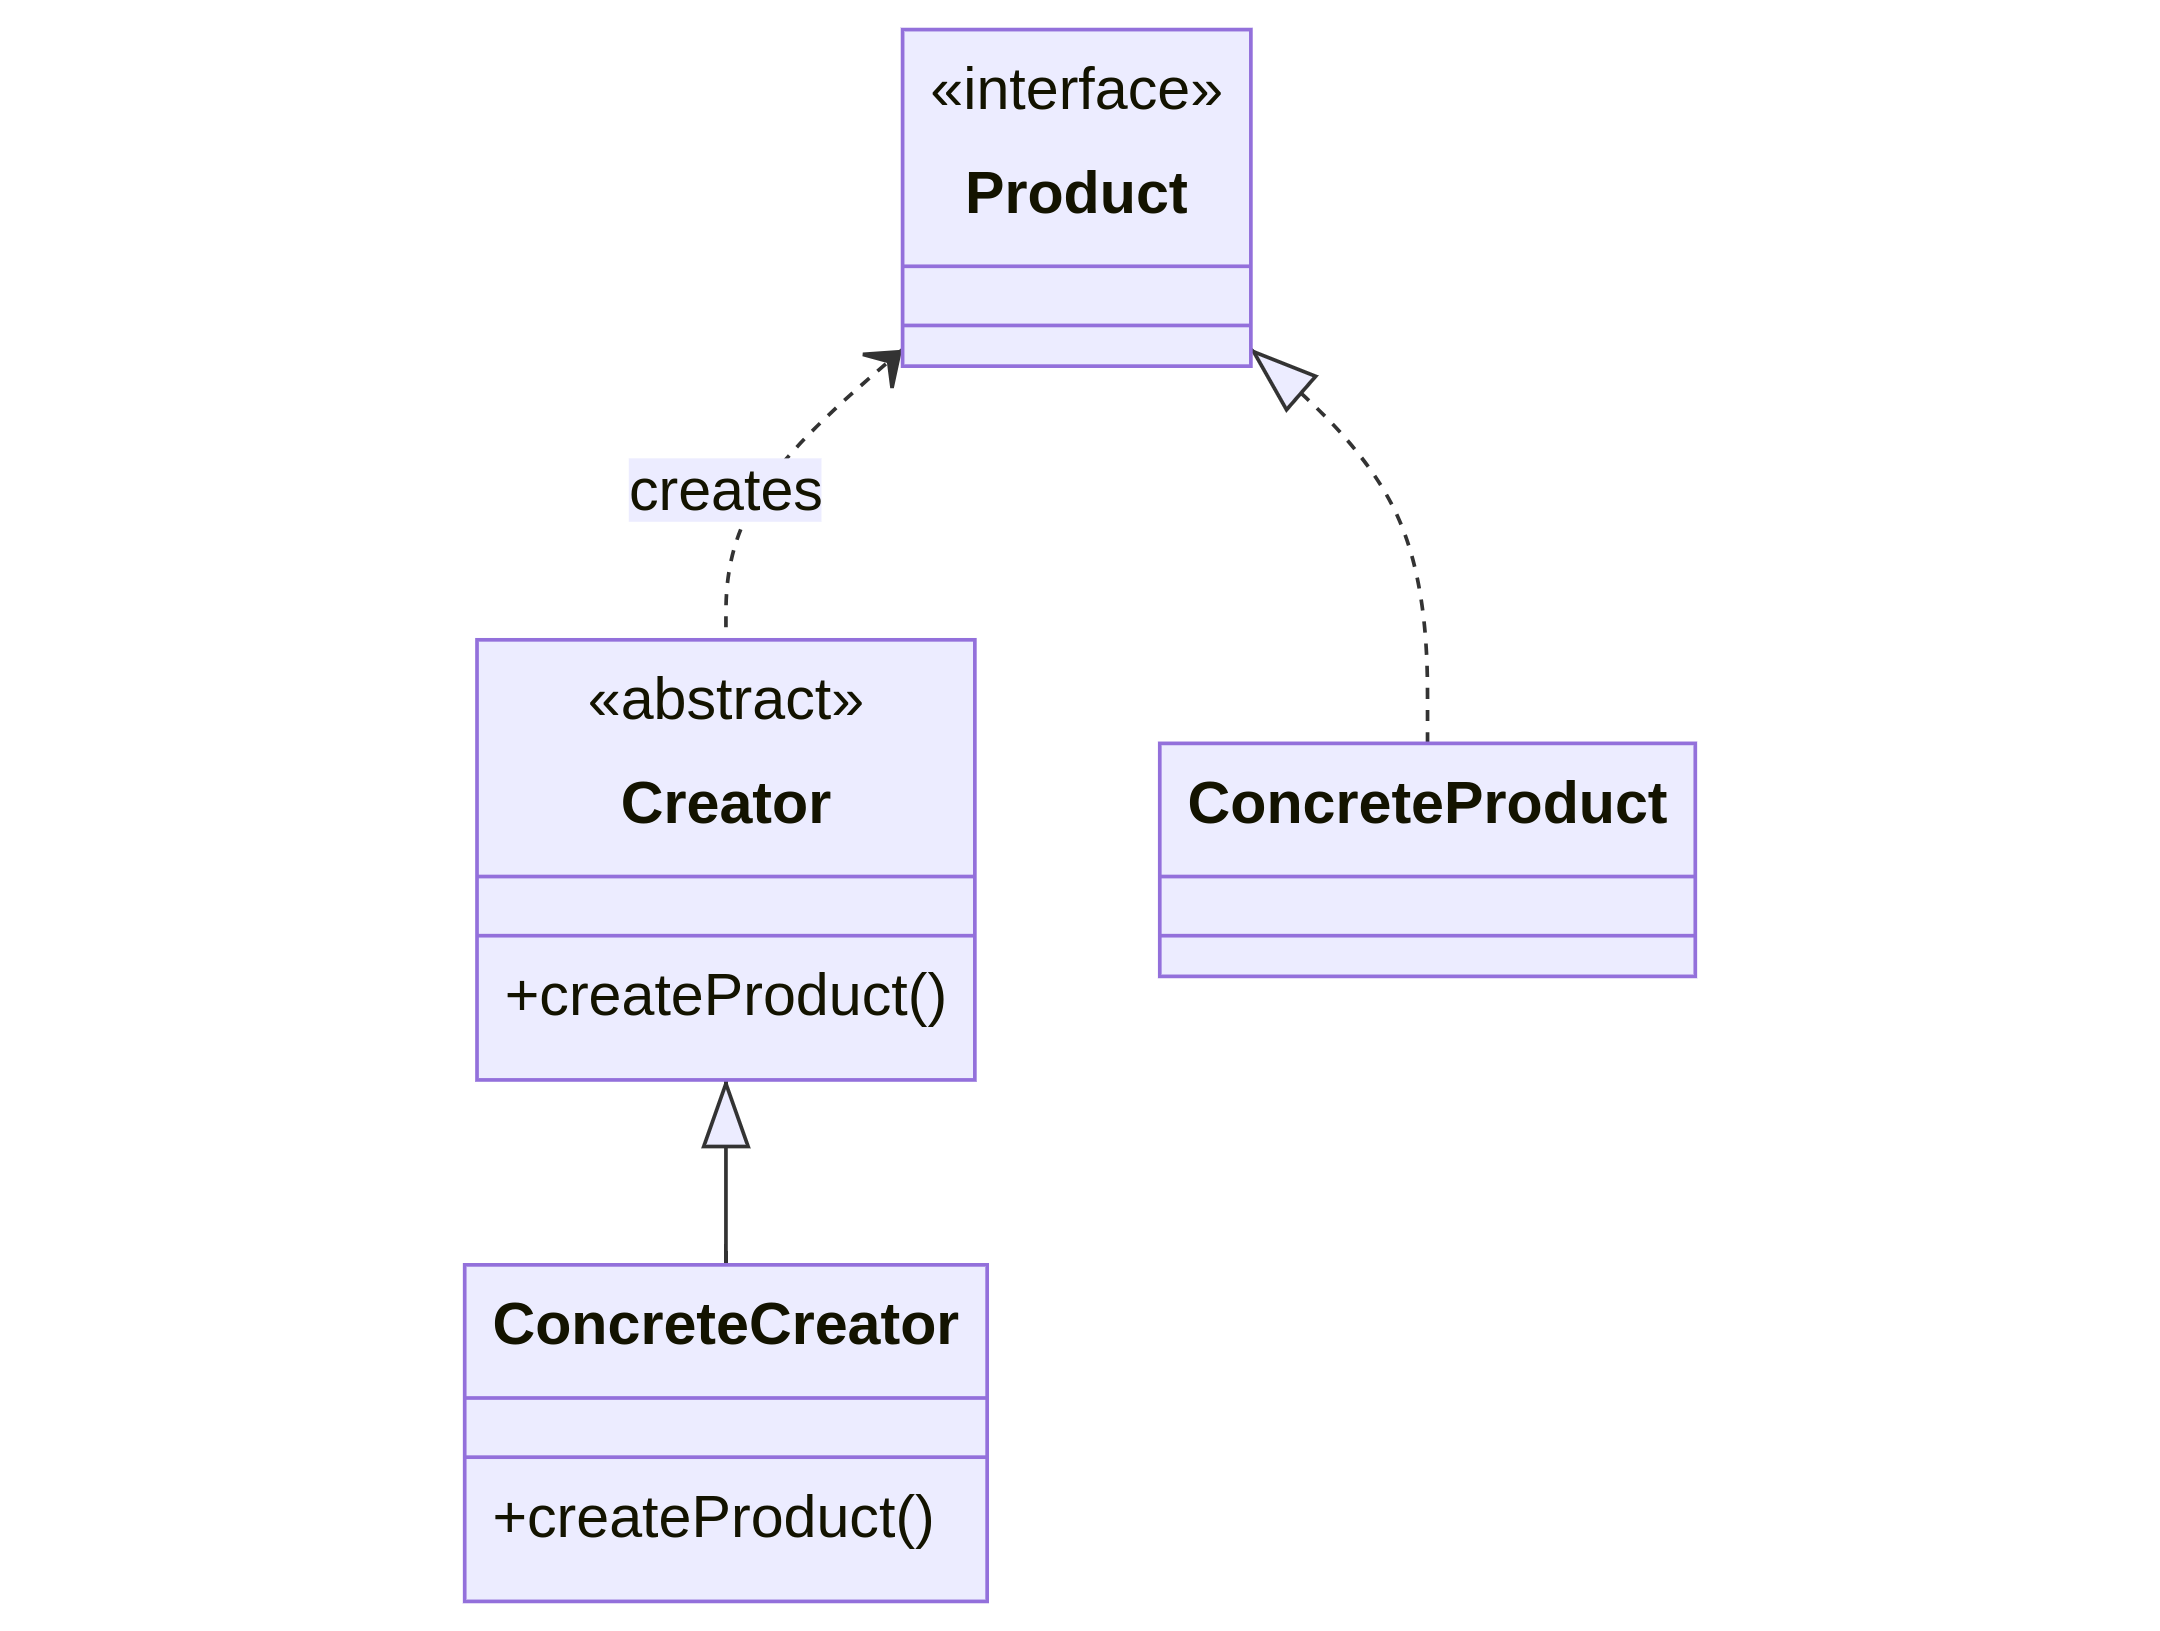
\includegraphics[width=0.75\linewidth]{images/patterns/factory-method-class.png}
	\caption{Klassendiagramm Factory Method}
	\label{fig:factory-method-class}
\end{figure}

\subsubsection*{Konsequenzen}
Ein Objekt über eine Factory-Method zu erzeugen ist flexibler, als das Objekt direkt über den Konstruktor der Klasse zu instanziieren. Die erzeugende Klasse braucht nur das Interface des abstrakten `Creator` zu kennen und ist somit in der Lage beliebige konkrete Produkte über  deren korrespondierende konkrete `Creator` zu erzeugen. Hierbei fällt auf, dass die `Creator`-Klassenhierarchie die Produkt-Klassenhierarchie spiegelt. Für jeden Produkttyp existiert also auch eine `Creator`-Klasse. Daraus kann sich jedoch auch ein Nachteil ergeben. Zur Nutzung eines Produktes müssen nun stets zwei Subklassen definiert und zur Laufzeit ein weiteres Objekt erstellt werden. Das erhöht die Komplexität. 

